\chapter{混合(Blending)}
\begin{flushleft}
考虑图\ref{fig:10-1}。 首先绘制地形,绘制木箱,接着将地形和板条箱像素放在后面的缓冲区上。 然后,使用混合将水面绘制到后缓冲区(back buffer),以便水像素与地形混合,并在后缓冲区上放置像素,使地形和板条箱通过水显示。 在本章中,我们将研究混合技术,这些技术允许我们将当前光栅化的像素(所谓的源像素)与先前光栅化到后缓冲区的像素(所谓的目标像素)混合(组合)。这种技术使我们能够渲染半透明物体,如水和玻璃。\\
\end{flushleft}

\begin{figure}[h]
    \label{fig:10-1}
    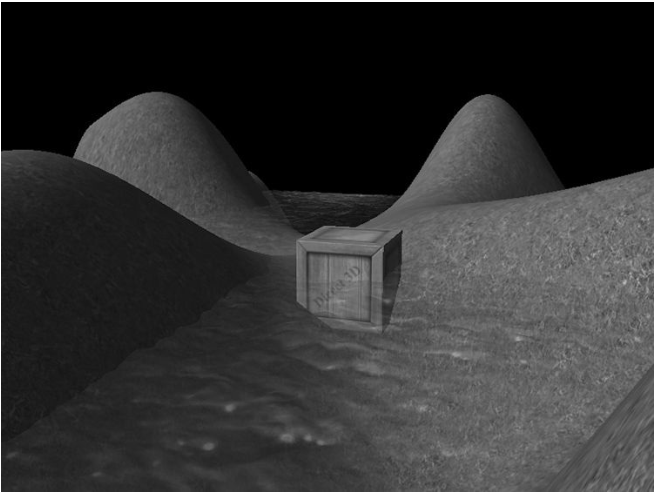
\includegraphics[width=\textwidth]{10-1}
    \centering
    \caption{半透明的水面。}
\end{figure}

\begin{flushleft}
~\\
NOTICE: 为了便于讨论,特别提到后缓冲区作为渲染目标。 但是,稍后将展示可以渲染到“屏幕外”渲染目标。 混合适用于这些渲染目标,目标像素是先前光栅化到这些屏幕外渲染目标的像素值。
~\\
{\large Objectives:}
\begin{itemize}
    \item 1.了解混合的工作原理以及如何将其与Direct3D一起使用。
    \item 2.了解Direct3D支持的不同混合模式。
    \item 3.了解如何使用alpha分量来控制基元(primitive)的透明度。
    \item 4.要了解如何通过使用HLSL clip 函数来阻止像素完全被绘制到后缓冲区。
\end{itemize}
\end{flushleft}

%-------- 10.1 --------
\section{混合公式(The Blending Equation)}
\begin{flushleft}
设$C_{src}$是当前光栅化的第$i$个像素(源像素)的像素着色器的颜色输出,并且设$C_{dst}$是当前在后缓冲器(目标像素)上的第$i$个像素的颜色。 如果没有混合,$C_{src}$将覆盖$C_{dst}$(假设它通过深度/模板测试(depth/stencil test))并成为第$i$个后缓冲区像素的新颜色。 但是通过混合,新颜色$C$将覆盖$C_{dst}$(即,混合颜色$C$将被写入后缓冲器的第$i$个像素)。 Direct3D使用以下混合公式来混合源像素和目标像素颜色:\\
\end{flushleft}

\begin{align*}
C=C_{src}\bigotimes F_{src}\boxplus C_{dst}\bigotimes F_{dst}
\end{align*}

\begin{flushleft}
颜色$F_{src}$(源混合因子)和$F_{dst}$(目标混合因子)可以是10.3节中描述的任何值,它们允许以各种方式修改原始源像素和目标像素,获得不同的效果。$\bigotimes$运算符是5.3.1节中定义的颜色向量的分量乘法; $\boxplus$运算符是10.2节中定义的任何二元运算符。\\

上述混合方程仅适用于颜色的RGB分量。alpha分量实际上由另一个单独公式处理:\\
\end{flushleft}

\begin{align*}
A=A_{src}F_{src}\boxplus A_{dst}F_{dst}
\end{align*}

\begin{flushleft}
等式基本相同,但混合因子和二元运算可能不同。 将RGB与alpha分离的动机很简单,可以独立处理它们,这使混合控制变得更灵活。\\
~\\
NOTICE: 与混合RGB分量相比,混合alpha分量的频率要低得多。 这主要是因为我们不关心后缓冲区alpha值。 如果您有一些需要目标alpha值的算法,则处理后缓冲区alpha值即可。
~\\
\end{flushleft}

%-------- 10.2 --------
\section{混合操作符(Blend Operations)}
\begin{flushleft}
二元运算符$\boxplus$由以下枚举类定义,用于混合公式运算:\\
\end{flushleft}

\begin{lstlisting}[mathescape]
typedef enum D3D12_BLEND_OP
{
    D3D12_BLEND_OP_ADD = 1, $C=C_{src}\bigotimes F_{src} + C_{dst}\bigotimes F_{dst}$
    D3D12_BLEND_OP_SUBTRACT = 2, $C=C_{dst}\bigotimes F_{dst} - C_{src}\bigotimes F_{src}$
    D3D12_BLEND_OP_REV_SUBTRACT = 3, $C=C_{src}\bigotimes F_{src} - C_{dst}\bigotimes F_{dst}$
    D3D12_BLEND_OP_MIN = 4, $C=min(C_{src},C_{dst})$
    D3D12_BLEND_OP_MAX = 5, $C=max(C_{src},C_{dst})$
} D3D12_BLEND_OP;
\end{lstlisting}

\begin{flushleft}
~\\
NOTICE: min/max 操作符忽略混合因子($F$)
~\\

这些运算符也适用于alpha混合公式。 此外,可以为RGB和alpha指定不同的运算符。 例如,可以添加两个RGB术语,但减去两个alpha术语:\\
\end{flushleft}

\begin{align*}
C&=C_{src}\bigotimes F_{src}+C_{dst}\bigotimes F_{dst}\\
A&=A_{src}F_{src}-A_{dst}F_{dst}
\end{align*}

\begin{flushleft}
最近添加到Direct3D的一个功能是使用逻辑运算符而不是上面的传统混合方程来混合源颜色和目标颜色。 可用的逻辑运算符如下:\\
\end{flushleft}

\begin{lstlisting}
typedef enum D3D12_LOGIC_OP
{
    D3D12_LOGIC_OP_CLEAR = 0,
    D3D12_LOGIC_OP_SET = ( D3D12_LOGIC_OP_CLEAR + 1 ),
    D3D12_LOGIC_OP_COPY = ( D3D12_LOGIC_OP_SET + 1 ),
    D3D12_LOGIC_OP_COPY_INVERTED = ( D3D12_LOGIC_OP_COPY + 1 ),
    D3D12_LOGIC_OP_NOOP = ( D3D12_LOGIC_OP_COPY_INVERTED + 1 ),
    D3D12_LOGIC_OP_INVERT = ( D3D12_LOGIC_OP_NOOP + 1 ),
    D3D12_LOGIC_OP_AND = ( D3D12_LOGIC_OP_INVERT + 1 ),
    D3D12_LOGIC_OP_NAND = ( D3D12_LOGIC_OP_AND + 1 ),
    D3D12_LOGIC_OP_OR = ( D3D12_LOGIC_OP_NAND + 1 ),
    D3D12_LOGIC_OP_NOR = ( D3D12_LOGIC_OP_OR + 1 ),
    D3D12_LOGIC_OP_XOR = ( D3D12_LOGIC_OP_NOR + 1 ),
    D3D12_LOGIC_OP_EQUIV = ( D3D12_LOGIC_OP_XOR + 1 ),
    D3D12_LOGIC_OP_AND_REVERSE = ( D3D12_LOGIC_OP_EQUIV + 1 ),
    D3D12_LOGIC_OP_AND_INVERTED = ( D3D12_LOGIC_OP_AND_REVERSE + 1 ),
    D3D12_LOGIC_OP_OR_REVERSE = ( D3D12_LOGIC_OP_AND_INVERTED + 1 ),
    D3D12_LOGIC_OP_OR_INVERTED = ( D3D12_LOGIC_OP_OR_REVERSE + 1)
} D3D12_LOGIC_OP;
\end{lstlisting}

\begin{flushleft}
请注意,不能同时使用传统的混合和逻辑运算符混合; 之孽那个选一个计算。 另请注意,为了使用逻辑运算符混合,渲染目标格式必须支持UINT变体的格式,否则您将收到如下错误:\\
\end{flushleft}
\begin{lstlisting}
D3D12 ERROR:
ID3D12Device::CreateGraphicsPipelineState: The render
target format at slot 0 is format (R8G8B8A8_UNORM). This
format does not support logic ops. The Pixel Shader
output signature indicates this output could be written,
and the Blend State indicates logic op is enabled for
this slot. [ STATE_CREATION ERROR #678:
CREATEGRAPHICSPIPELINESTATE_OM_RENDER_TARGET_DOES_NOT_SUPPORT_LOGIC_OPS]
D3D12 WARNING: ID3D12Device::CreateGraphicsPipelineState:
Pixel Shader output ‘SV_Target0’ has type that is NOT
unsigned int, while the corresponding Output Merger
RenderTarget slot [0] has logic op enabled. This happens
to be well defined: the raw bits output from the shader
will simply be interpreted as UINT bits in the blender
without any data conversion. This warning is to check
that the application developer really intended to rely on
this behavior. [ STATE_CREATION WARNING #677:
CREATEGRAPHICSPIPELINESTATE_PS_OUTPUT_TYPE_MISMATCH]
\end{lstlisting}

%-------- 10.3 --------
\section{混合因子(Blend Factors)}
\begin{flushleft}
通过为源和目标混合因子设置不同的组合以及不同的混合运算符,可以实现许多不同的混合效果。 我们将在10.5节中说明一些组合,但您需要尝试其他组合以了解它们的作用。以下列表描述了适用于$F_{src}$和$F_{dst}$的基本混合因子。有关其他一些高级混合因子,请参阅SDK文档中的D3D12\_BLEND枚举类型。设$C_{src}=(r_{s},g_{s},b_{s})$,$A_{src}=a_{s}$(从像素着色器输出的RGBA值),$C_{dst}=(r_{d},g_{d},b_{d})$,$A_{dst}=a_{d}$(RGBA值已经存储在渲染目标中),$F$为$F_{src}或$F_{dst}$,我们有:\\
~\\
D3D12\_BLEND\_ZERO: $F=(0,0,0) and F=0$\\
D3D12\_BLEND\_ONE: $F=(1,1,1) and F=1$\\
D3D12\_BLEND\_SRC\_COLOR: $F=(r_{s},g_{s},b_{s})$\\
D3D12\_BLEND\_INV\_SRC\_COLOR: $F_{src}=(1−r_{s}, 1−g_{s},1−b_{s})$\\
D3D12\_BLEND\_SRC\_ALPHA: $F=(a_{s},a_{s},a_{s}) and F=a_{s}$\\
D3D12\_BLEND\_INV\_SRC\_ALPHA: $F=(1−a_{s},1−a_{s},1−a_{s}) and F=(1−a_{s})$\\
D3D12\_BLEND\_DEST\_ALPHA: $F=(a_{d},a_{d},a_{d}) and F=a_{d}$\\
D3D12\_BLEND\_INV\_DEST\_ALPHA: $F=(1−a_{d},1−a_{d},1−a_{d}) and F=(1−a_{d})$\\
D3D12\_BLEND\_DEST\_COLOR: $F=(r_{d},g_{d},b_{d})$\\
D3D12\_BLEND\_INV\_DEST\_COLOR: $F=(1−r_{d},1−g_{d},1−b_{d})$\\
D3D12\_BLEND\_SRC\_ALPHA\_SAT: $F=(a^{'}_{s},a^{'}_{s},a^{'}_{s}) and F=a^{'}_{s} where a^{'}_{s}=clamp(a_{s},0,1)$\\

D3D12\_BLEND\_BLEND\_FACTOR: $F=(r,g,b) and F=a$\\
其中颜色$(r,g,b,a)$被提供给 ID3D12GraphicsCommandList::OMSetBlendFactor 方法的第二个参数。 这允许您指定要直接使用的混合因子颜色; 在更改混合状态之前,它是不变的。\\

D3D12\_BLEND\_INV\_BLEND\_FACTOR: $F=(1-r,1-g,1-b) and F=1-a$\\
其中颜色$(r,g,b,a)$被提供给 ID3D12GraphicsCommandList::OMSetBlendFactor 方法的第二个参数。这允许您指定要直接使用的混合因子颜色; 在更改混合状态之前,它是不变的。\\
~\\
所有上述混合因子都适用于RGB混合公式。对于alpha混合等式,不允许以 \_COLOR 结尾的混合因子。\\
~\\
NOTICE: $clamp$函数定义如下:\\
\end{flushleft}

\begin{align*}
clamp(x,a,b)=\left\{\begin{matrix}
x,a\leq x \leq b\\ 
a,x<a\\ 
b,x>b
\end{matrix}\right.
\end{align*}

\begin{flushleft}
~\\
NOTICE: 我们可以使用以下函数设置混合因子颜色:\\
\end{flushleft}
\begin{lstlisting}
void ID3D12GraphicsCommandList::OMSetBlendFactor(const FLOAT BlendFactor [4]); 
\end{lstlisting}

\begin{flushleft}
传递 nullptr 会恢复默认的混合因子$(1,1,1,1)$。
~\\
\end{flushleft}

%-------- 10.4 --------
\section{混合状态(Blend State)}
\begin{flushleft}

\end{flushleft}









